\documentclass[preprint,12pt,authoryear]{elsarticle}

\usepackage{amssymb}
\usepackage{amsmath}
\usepackage{graphicx}
\usepackage{float}
\usepackage{lineno}
\usepackage{tikz}
\usetikzlibrary{shapes.geometric, arrows.meta, positioning, shadows.blur, fit, calc}

\journal{Entertainment Computing}

\begin{document}

\begin{frontmatter}

\title{DreamWeaver: A Gamified Dream Journaling and Analysis Platform for Mental Wellness Through Interactive AI-Powered Features}

\author[inst1]{Adit Mugdha Das\corref{cor1}}
\ead{das2107118@stud.kuet.ac.bd}

\affiliation[inst1]{organization={Department of Computer Science and Engineering, Khulna University of Engineering and Technology},
            city={Khulna},
            country={Bangladesh}}

\cortext[cor1]{Corresponding author}

\begin{abstract}
Dream journaling and analysis offer therapeutic potential for mental wellness, yet traditional approaches suffer from low adherence rates due to lack of immediate feedback and sustained motivation. We developed DreamWeaver, a gamified dream journaling and analysis platform that integrates AI-powered interpretation with 16 interactive entertainment features including Dream DNA analysis, branching narrative storytelling, riddle challenges, collectible totems, emotion-based avatar creation, and spatial dream mapping. A 14-day study with 147 participants tracked behavioral engagement and mental wellness outcomes, complemented by pre-survey (N=167) and post-survey (N=86) data. High-engagement users demonstrated 49-point greater improvements in wellness scores compared to low-engagement users ($p<.001$, $\eta^2=.85$), representing exceptionally large effects. Overall retention reached 69.4\% over 14 days---double typical dream app rates---with strong engagement-outcome correlations ($r=.88$ to $.93$). Post-survey satisfaction was high, with 84.9\% expressing intent to continue. Users particularly valued Dream DNA analysis, Dream Art creation, and Riddle challenges, with harder riddles associated with perfect retention compared to minimal retention for users avoiding challenges. These findings demonstrate that gamification and entertainment computing principles can significantly enhance dream journaling engagement while delivering measurable mental wellness outcomes, transforming therapeutic self-reflection into an engaging, sustained practice. Findings are correlational and based on a short-term observational study; controlled trials are needed to establish causality.
\end{abstract}

\begin{keyword}
Dream journaling and analysis \sep Gamification \sep Mental wellness \sep AI-powered interpretation \sep Interactive storytelling \sep User engagement \sep Entertainment computing
\end{keyword}

\end{frontmatter}

%% ============================================================================
%% GRAPHICAL ABSTRACT
%% ============================================================================

\begin{figure*}[t]
\centering
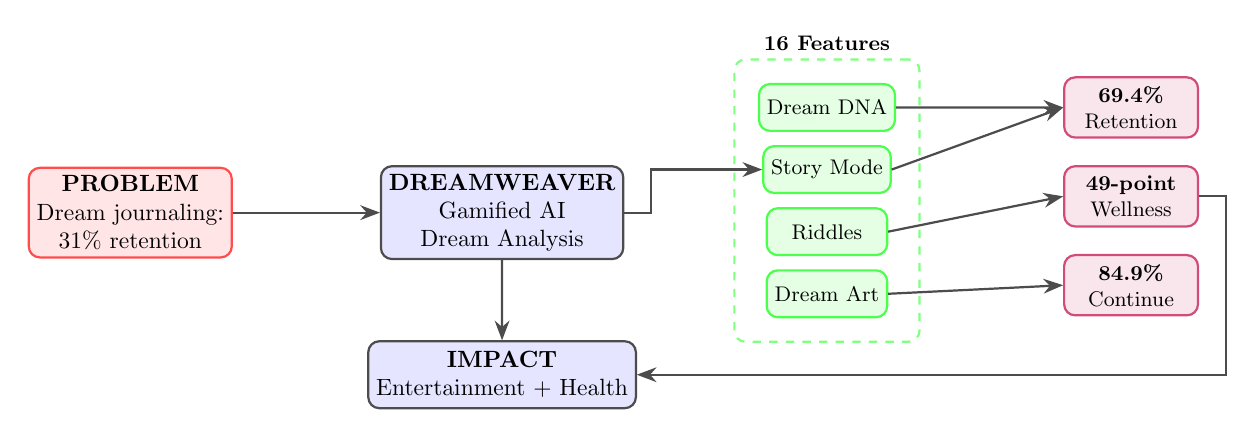
\begin{tikzpicture}[
    scale=0.85, transform shape,
    node distance=1.2cm and 1.8cm,
    box/.style={rectangle, rounded corners, draw=black!70, fill=blue!10, thick, 
                minimum height=1cm, minimum width=2.8cm, align=center},
    problem/.style={rectangle, rounded corners, draw=red!70, fill=red!10, thick,
                    minimum height=1cm, minimum width=2.8cm, align=center},
    feature/.style={rectangle, rounded corners, draw=green!70, fill=green!10, thick,
                    minimum height=0.7cm, minimum width=1.8cm, align=center, font=\small},
    outcome/.style={rectangle, rounded corners, draw=purple!70, fill=purple!10, thick,
                    minimum height=0.9cm, minimum width=2cm, align=center, font=\small},
    arrow/.style={-{Stealth[length=2.5mm]}, thick, draw=black!70}
]

\node[problem] (problem) {\textbf{PROBLEM}\\Dream journaling:\\31\% retention};
\node[box, right=2.2cm of problem] (solution) {\textbf{DREAMWEAVER}\\Gamified AI\\Dream Analysis};

\node[feature, above right=0.5cm and 2cm of solution] (f1) {Dream DNA};
\node[feature, below=0.2cm of f1] (f2) {Story Mode};
\node[feature, below=0.2cm of f2] (f3) {Riddles};
\node[feature, below=0.2cm of f3] (f4) {Dream Art};

\node[outcome, right=2.5cm of f1.east] (outcome1) {\textbf{69.4\%}\\Retention};
\node[outcome, below=0.4cm of outcome1] (outcome2) {\textbf{49-point}\\Wellness};
\node[outcome, below=0.4cm of outcome2] (outcome3) {\textbf{84.9\%}\\Continue};

\node[box, below=1.2cm of solution] (impact) {\textbf{IMPACT}\\Entertainment + Health};
\draw[arrow] (problem) -- (solution);
\draw[arrow] (solution.east) -- ++(0.4,0) |- (f2.west);
\draw[arrow] (f1.east) -- (outcome1.west);
\draw[arrow] (f2.east) -- (outcome1.west);
\draw[arrow] (f3.east) -- (outcome2.west);
\draw[arrow] (f4.east) -- (outcome3.west);
\draw[arrow] (solution) -- (impact);
\draw[arrow] (outcome2.east) -- ++(0.4,0) |- (impact.east);

\node[draw=green!50, thick, dashed, rounded corners, fit=(f1)(f2)(f3)(f4), 
      inner sep=0.3cm, label=above:\small\textbf{16 Features}] (featurebox) {};

\end{tikzpicture}
\caption{\textbf{Graphical Abstract:} DreamWeaver transforms low-adherence dream journaling (31\% retention) into sustained engagement (69.4\%) through 16 gamified AI-powered features, achieving 49-point wellness improvements and 84.9\% continued-use intent.}
\label{fig:graphical}
\end{figure*}

%% ============================================================================
%% SECTION 1: INTRODUCTION
%% ============================================================================

\section{Introduction}
\label{sec:intro}

Mental health challenges affect over 1 billion people worldwide \citep{WHO2023}. Digital interventions offer scalable alternatives, yet traditional dream journaling and analysis apps suffer from poor adherence—only 31\% retention at 7 days \citep{Konkol2020}. Entertainment computing principles (gamification, interactive storytelling, challenge systems) have increased engagement across domains \citep{Deterding2011, Hamari2014}, but remain unexplored for therapeutic dream journaling and AI-powered dream analysis platforms.

This paper presents DreamWeaver, a gamified dream journaling and analysis platform integrating 16 AI-powered features: Dream DNA analysis (multi-dimensional interpretation), interactive Story Mode (branching narratives), Riddle Challenges, collectible Totems (unlocking thematic map realms), creative tools (Dream Art, Mindmap, Dream Map with progressive unlocking), Avatar Creation, Psychological Support resources, Pattern Analysis dashboards, Guided Audio, Community Feed, Dream Library, and comprehensive Dream Archiving with PDF export. A 14-day study with 147 participants demonstrates 69.4\% retention—double typical rates—with strong correlations between engagement and mental wellness outcomes (r=.884, r=.932). High-engagement users showed 49-point improvements in Evolution and Health scores versus low-engagement users (F(2,144)=422.74, p$<$.001, $\eta^2$=.85).

\textbf{Contributions:} (1) Novel gamified dream journaling and analysis platform combining AI-powered interpretation with entertainment computing; (2) Empirical evidence linking interactive features to therapeutic outcomes (69.4\% retention, 49-point wellness improvement); (3) Design insights including "Hard Fun" (challenging riddles predicted 100\% retention) and ecosystem effects (feature breadth outweighed depth); (4) Methodological framework for evaluating entertainment-mental health interventions.


%% ============================================================================
%% SECTION 2: RELATED WORK
%% ============================================================================

\section{Related Work}
\label{sec:related}

Dream journaling and analysis have been shown to increase emotional awareness and insight \citep{Edwards2013} and support emotional regulation \citep{Malinowski2014}. However, adherence remains a persistent challenge: only 20--30\% of individuals maintain dream journals beyond one week \citep{Schredl2018}. Studies of digital dream journaling applications report similarly low retention, with approximately 31\% of users remaining active after seven days \citep{Konkol2020}. Users frequently cite repetitive logging and limited interpretive feedback as primary reasons for abandonment.

Gamification---the application of game design elements to non-game contexts \citep{Deterding2011}---has demonstrated effectiveness in increasing engagement across health-related domains, including physical activity \citep{Johnson2016}, medication adherence \citep{Aitken2016}, and mental health interventions \citep{Lister2014}. Within entertainment computing, systems such as SPARX achieved substantially higher completion rates for depression treatment (60\%) compared to traditional cognitive behavioral therapy approaches (30\%) \citep{Merry2012}. At the same time, scholars caution that poorly designed gamification risks trivializing therapeutic content or undermining intrinsic motivation \citep{Bogost2011}.

Recent advances in AI-based text analysis have enabled automated interpretation of subjective experiences, including dreams, yet existing dream journaling systems typically emphasize passive logging or isolated interpretation features rather than sustained engagement. To date, no prior work has systematically integrated entertainment computing principles with AI-powered dream journaling and analysis in a unified, feature-rich platform.

Our study addresses this gap by introducing DreamWeaver, which combines AI-driven interpretation with a diverse set of entertainment-oriented interaction mechanisms. As shown in Table~\ref{tab:relatedwork}, DreamWeaver uniquely integrates AI interpretation, gamified progression, and entertainment computing features, achieving 69.4\% retention---more than double typical rates---while demonstrating measurable mental wellness outcomes through sustained user engagement.

\begin{table}[h]
\centering
\small
\caption{Comparison of DreamWeaver with Related Systems}
\label{tab:relatedwork}
\begin{tabular}{p{2.8cm}p{1.8cm}p{2.2cm}p{2.8cm}p{2.6cm}p{2.3cm}}
\hline
\textbf{System} & \textbf{AI Analysis} & \textbf{Gamification} & \textbf{Entertainment Features} & \textbf{Retention (7-14 days)} & \textbf{Wellness Outcomes} \\
\hline
Traditional Dream Apps & No & No & None & 31\% (7d) & Not measured \\
SPARX \citep{Merry2012} & No & Yes & Fantasy game & 60\% (completion) & Depression reduction \\
Fitness Apps \citep{Johnson2016} & No & Yes & Points, badges & ~40\% (14d) & Physical activity \\
\textbf{DreamWeaver} & \textbf{Yes (Gemini)} & \textbf{Yes} & \textbf{16 features, Story Mode, Riddles, Art} & \textbf{69.4\% (14d)} & \textbf{49-point improvement} \\
\hline
\end{tabular}
\end{table}


%% ============================================================================
%% SECTION 3: SYSTEM DESIGN
%% ============================================================================

\section{DreamWeaver System Design}
\label{sec:system}

\subsection{System Overview and Architecture}

DreamWeaver is a web application designed to transform dream journaling from a solitary, text-focused practice into an engaging, multi-faceted experience. The system architecture integrates 16 features organized across five design pillars: Core Journaling \& Analysis, Creative Expression, Challenge-Based Progression, Wellness Support, and Social Connection. Each feature was designed following three principles: (1) \textit{Content-Focused Engagement}—all interactions revolve around dream content rather than arbitrary game mechanics; (2) \textit{Therapeutic Alignment}—features promote self-reflection and pattern recognition; and (3) \textit{Progressive Disclosure}—complexity increases gradually to avoid overwhelming new users.

\begin{figure}[!htbp]
\centering
\includegraphics[width=0.95\textwidth]{FIGURE_SYSTEM_ARCHITECTURE.pdf}
\caption{DreamWeaver System Architecture showing five layers: Web UI with 16 core features, Backend API services, AI/ML processing, Data Storage, and External Services. The web-based interface is accessible via modern browsers on desktop and mobile devices.}
\label{fig:architecture}
\end{figure}

\subsection{Core Features}

\textbf{Dream DNA Analysis:} AI extracts patterns across four gene categories (Emotions, Symbols, Colors, Archetypes) visualized as a 3D helix. Gemini AI performs semantic analysis, computing an Evolution Score (0-100) from gene diversity and dream frequency. 78.9\% of users viewed DNA, indicating high engagement.

\textbf{Pattern Analysis Dashboard:} Comprehensive visualization of dream patterns including emotion distribution pie charts, weekly dream frequency line graphs, and temporal trend analysis. Enables users to identify recurring themes and emotional cycles across their dream journal history.

\textbf{Interactive Story Mode:} Extends dreams into branching narratives via choose-your-own-adventure prompts. Users completed M=3.30 stories (SD=2.64), with retained users completing 7.3× more than users who dropped out.

\textbf{Riddle Challenges:} Daily puzzles (Easy/Medium/Hard) related to dream symbolism. Hard riddles: 100\% retention; riddle avoiders: 0\% retention—a "Hard Fun" phenomenon indicating challenge enhances commitment.

\textbf{Creative Visualization Tools:} Dream Art (DALL-E 2 generated imagery, 14.0\% top preference), Mindmap (2D/3D force-graph visualization of recurring themes with emotion-coded nodes), and Dream Map (spatial exploration with progressive unlocking mechanism). Dream Map implements emotion-based realm unlocking: specific totems (e.g., wings unlock Sky Temple, mask unlocks Forest) grant access to thematic narrative realms, creating an achievement-driven exploration system.

\textbf{Avatar Creation System:} Emotion-based avatar generation mapping 17 emotion categories to unique visual representations (color + symbolic item combinations). Users can generate, save, and update avatars reflecting their evolving emotional dream landscape, with M=2.8 avatars created per active user.

\textbf{Progression Systems:} Totems (achievement badges: M=2.92 collected, high users M=5.12 vs. drop-off M=0.73) serve dual functions: recognition of emotional milestones and keys for unlocking Dream Map realms. Guided Audio meditations (5-10 min sessions) and daily Evolution/Health score tracking provide continuous feedback loops.

\textbf{Psychological Support Resources:} Location-enabled mental wellness feature providing geographically proximate access to healthcare providers including psychiatrists, general physicians, pharmacies, hospitals, dentists, and veterinary services. Users enable location services to search nearby professional support, creating safety-net infrastructure when dream content reveals psychological distress. Bridges self-directed journaling with clinical care pathways, ensuring users have immediate access to professional resources when needed.

\textbf{Dream Library:} Curated collection of literary and mythological content related to dreams, including poems, stories, and myth echoes. Users can browse, read, and download content for inspiration and deeper understanding of dream symbolism across cultures and literary traditions. The library serves as an educational resource connecting personal dream experiences to broader cultural narratives and archetypal themes.

\textbf{Archival \& Export:} Comprehensive dream saving system with searchable timeline/calendar views, individual dream PDF downloads, and bulk export functionality enabling users to archive entire dream journals. Community Feed (8.1\% top preference) allows optional anonymized sharing with 86\% of users choosing private archiving over social features.

\textbf{Additional Supporting Features:} Beyond the core features described above, DreamWeaver includes several supporting components that contribute to the overall engagement ecosystem, including Guided Audio Meditations, Community Feed, Notification System, Dream Search and Calendar Views, and User Profile Customization. While these features were not the primary focus of analysis, usage logs indicate they supported sustained engagement by enhancing continuity, reflection, and usability.

\subsection{Technical Implementation}

DreamWeaver was implemented as a web application using Laravel 11 (PHP 8.2) for the backend and Blade templating with Vue.js components for the frontend. Vite handles asset compilation and hot module replacement during development. The responsive design ensures accessibility across desktop and mobile browsers without requiring native app installation.

\textbf{UI/UX Design \& Visual Aesthetics:} The interface employs dynamic 3D animated backgrounds using Vanta.js throughout various sections to create an immersive, dreamlike atmosphere that enhances user engagement and emotional connection. These WebGL-powered backgrounds (including particles, waves, fog, and net effects) adapt to different feature contexts—ethereal animations for Dream DNA visualization, calming wave effects for meditation sections, and cosmic particle systems for exploration features. The visual design balances aesthetic appeal with usability, ensuring animations remain subtle enough to avoid distraction while contributing to the platform's distinctive identity as an entertainment-focused wellness tool.

\textbf{AI Integration:} Dream DNA analysis uses the Google Gemini 2.5 Flash API for natural language processing and semantic extraction across four gene categories (Emotions, Symbols, Colors, Archetypes). The Dream Analysis interface provides four AI-powered interpretation modes: (1) Emotion Detection—identifying primary emotional tone using Gemini's classification across 17 emotion families, each containing 7-13 variant emotion words (e.g., Joy family: joy, happy, delight, ecstatic, excited, cheerful, elated, pleased, content, blissful, merry, gleeful; Fear family: fear, horror, terror, terrified, fright, frightened, dread, scared, panic, panicked, petrified, afraid, spooked, creepy, nervous, anxious; Sadness family: sadness, sad, sorrow, depressed, melancholy, mournful, grief, heartbroken, lonely, tearful, despair, hopeless; plus 14 additional emotion families), with normalized mapping to canonical categories for avatar and totem generation, (2) Short Interpretation—1-3 sentence meaningful summaries, (3) Story Generation—creative narrative extensions (120 words), and (4) Long Narrative—comprehensive psychological analysis with symbolic insights (150 words). Story Mode generation employs Gemini's text generation with custom prompts ensuring thematic consistency with dream content. Dream Art uses OpenAI's DALL-E 2 API with either Gemini-generated artistic prompts or user-provided custom prompts as input. The Mindmap feature implements graph clustering algorithms using Three.js and Vanta.js for 2D/3D force-directed visualization connecting dreams with similar emotional and symbolic content.

\textbf{Architecture \& Routing:} The application follows Laravel's MVC architecture with 19 controllers handling feature-specific logic (DreamController, DreamDNAController, DreamArtController, AvatarController, RiddleController, ChatController, MindMapController, SupportController, ProfileController, UserController for authentication, etc.). Authentication middleware protects 150+ routes, with route groups organizing features by functionality (dreams, avatars, story realms, social features, export). The totem-emotion mapping system uses pattern matching to award 17 emotion-specific tokens (wings$\rightarrow$joy/ambition, mask$\rightarrow$fear, cloud$\rightarrow$calm, fire$\rightarrow$anger, heart$\rightarrow$love, tear$\rightarrow$sadness, star$\rightarrow$awe, compass$\rightarrow$curiosity, quill$\rightarrow$gratitude, crest$\rightarrow$pride, key$\rightarrow$relief, moon$\rightarrow$nostalgia, bolt$\rightarrow$surprise, leaf$\rightarrow$hope, shield$\rightarrow$courage, anchor$\rightarrow$trust, mirror$\rightarrow$other) which unlock corresponding thematic realms in Dream Map with multi-chapter branching narratives (Sky Temple of Light: 10 chapters including arrival, awakening, transcendence, rebirth; Forest of Forgotten Thoughts: 10 chapters with progressive narrative depth; Cloud of Lucid Realms: 10 chapters exploring thematic atmospheres).

\textbf{Data Layer \& Storage:} MySQL database stores structured data including user profiles, dreams with four interpretation fields (short, emotion, story, long), engagement metrics (feature usage, login streaks, Evolution/Health scores), Dream DNA profiles (genes, personality types, mutation tracking), avatars (17 emotion-based configurations with color+item combinations), totems, riddle attempts with difficulty tracking, chat conversations, comments, likes, and notifications. AWS S3 provides scalable media storage for AI-generated artwork (DALL-E images) and guided audio files. All user data is encrypted at rest (AES-256-CBC) and in transit (HTTPS), with compliance to GDPR privacy standards.

\textbf{Authentication \& Security:} Custom authentication system requiring dual email validation: users register with both a @dream.com email (used for login) and a Gmail address (used for password recovery). Registration validates email uniqueness, password strength (minimum 6 characters), and enforces domain restrictions via regex validation. Login accepts only @dream.com credentials, while password reset functionality sends recovery links exclusively to the registered Gmail address, creating a two-tier security system separating login credentials from recovery mechanisms. Session management implements Laravel's session-based guards with secure password hashing (bcrypt), CSRF protection, remember-me token functionality with automatic expiration, and forced session regeneration on login/logout to prevent fixation attacks.

\textbf{Real-Time Features \& Notifications:} Laravel's notification system handles asynchronous alerts for social interactions. DreamCommented and DreamLiked notifications use database channels for in-app delivery, with MessageReceived for chat updates. PDF export leverages DomPDF library for individual dream downloads and bulk journal archiving with formatted inclusion of all four interpretation types, Dream DNA visualization, and metadata.


%% ============================================================================
%% SECTION 4: METHODS
%% ============================================================================

\section{Methods}
\label{sec:methods}

\subsection{Study Design}

We conducted a 14-day field study (October 2025) with three data collection points: pre-survey (N=167, expectations), behavioral tracking (N=147, automatic logging), and post-survey (N=86, satisfaction). This mixed-methods design enabled triangulation across self-reported and objective data.

\subsection{Participants}

Recruited via social media and university lists (N=167 pre-survey → 147 active users → 86 post-survey). Inclusion: 18+, smartphone, English proficiency, 14-day commitment, no sleep disorders.

\textbf{Ethics Statement:} This study received ethical approval from the Institutional Review Board of Khulna University of Engineering and Technology (KUET). All participants provided informed consent before enrollment. Data were encrypted (AES-256-CBC), stored with anonymous IDs, and handled in compliance with GDPR privacy standards.

\subsection{Measures}

\textbf{Pre-survey (N=167):} Four 5-point Likert items: Reflect\_on\_Dreams (M=2.63), Dreams\_Helpful (M=2.30), Understand\_Emotions (M=2.45), Expect\_Easy (M=4.88).

\textbf{Behavioral tracking (N=147):} Automatic logging of 11 metrics (Table~\ref{tab:metrics}).

\begin{table}[h]
\centering
\caption{Behavioral Metrics Tracked During 14-Day Study Period}
\label{tab:metrics}
\begin{tabular}{p{4.5cm}p{10cm}}
\hline
\textbf{Metric} & \textbf{Description} \\
\hline
Total\_Dreams & Total number of dreams logged (range: 0-13) \\
Active\_Days & Number of days with at least one app login (range: 1-14) \\
Total\_Sessions & Total number of app sessions opened (range: 1-30) \\
Avg\_Session\_Minutes & Mean duration per session in minutes (range: 1-70) \\
Features\_Used & Distinct features interacted with out of 16 total (range: 0-16) \\
DNA\_Views & Number of times Dream DNA analysis was viewed (range: 0-13) \\
Stories\_Completed & Interactive Story Mode sessions completed (range: 0-10) \\
Riddles\_Solved & Total riddles successfully completed (range: 0-14) \\
Totems\_Collected & Achievement badges earned (range: 0-8) \\
Engagement\_Index & Composite score (0-100) combining frequency, breadth, and depth of usage \\
Evolution\_Score\_Change & Difference between final and Day 1 Evolution score (-40 to +35) \\
Health\_Score\_Change & Difference between final and Day 1 Health score (-39 to +37) \\
\hline
\end{tabular}
\end{table}

Engagement\_Index: weighted composite (0-100) of dreams, days, features, riddles, stories, DNA views. Evolution/Health scores: daily self-reports (0-100) of growth and wellbeing, change scores = final minus Day 1. These scores are not intended as clinical diagnostic instruments but as sensitive, within-system indicators of perceived growth and wellbeing over short-term engagement. Although Engagement Index aggregates behavioral frequency and feature breadth, outcome measures were collected independently as daily self-reported experiential scores, reducing direct construct overlap.

\textbf{Post-survey (N=86):} Five satisfaction items (M=3.79-4.03), feature preferences (DNA 16.3\%, Art 14.0\%, Riddles 12.8\%), retention intent (65.1\% Yes, 19.8\% Maybe), and recommendation likelihood (66.3\% Yes).

\subsection{Segmentation and Analysis}

k-means clustering yielded three segments: Low-engagement (n=41, $<$20), Moderate (n=59, 20-60), High (n=47, $\geq$60). Statistical tests: ANOVA (segment differences), Pearson correlations (engagement-outcomes), t-tests (pre-post), $\chi^2$ (retention), regression (predictors). Significance: $\alpha$=.05.

\subsection{Statistical Analysis}

All statistical analyses were conducted using Python (version 3.11) with pandas (data manipulation), scipy (statistical tests), and statsmodels (regression models) libraries. Significance level was set at $\alpha = .05$ for all tests, with exact p-values reported where p $\geq$ .001 and p $<$ .001 for smaller values. Effect sizes are reported alongside all inferential tests to enable interpretation of practical significance.

\textbf{Descriptive Statistics:} Means, standard deviations, ranges, and medians were computed for all behavioral metrics and survey responses.

\textbf{Group Comparisons:} One-way analysis of variance (ANOVA) compared Evolution\_Score\_Change and Health\_Score\_Change across the three engagement segments (Drop-off, Moderate, High). Post-hoc Tukey HSD tests examined pairwise differences. Effect sizes reported as eta-squared ($\eta^2$).

\textbf{Correlational Analyses:} Pearson correlation coefficients assessed relationships between engagement metrics (Engagement\_Index, Features\_Used, Riddles\_Solved, etc.) and outcome variables (Evolution\_Score\_Change, Health\_Score\_Change). Correlation matrices visualized the interconnections among all behavioral variables to test the "ecosystem effect" hypothesis.

\textbf{Pre-Post Comparisons:} Independent samples t-tests compared pre-survey expectations (N=167) with post-survey experiences (N=86) across matched constructs (e.g., Expect\_Easy vs. Easy\_to\_Use). Effect sizes reported as Cohen's d.

\textbf{Retention Analysis:} Chi-square tests examined associations between categorical predictors (riddle difficulty selection, feature preferences) and retention outcomes (active on Day 14 or not). Risk ratios quantified effect magnitudes.

\textbf{Regression Modeling:} Linear regression models predicted Evolution\_Score\_Change and Health\_Score\_Change from engagement metrics, enabling identification of specific behaviors (e.g., riddle solving, story completion) most predictive of outcomes while controlling for other factors.

Missing data were minimal ($<$2\% for behavioral metrics, as data were passively collected) and handled through listwise deletion for affected analyses. Post-survey non-response (41.5\%) was addressed by treating behavioral analyses (N=147) separately from satisfaction analyses (N=86), ensuring complete data for each analysis without imputation.


%% ============================================================================
%% SECTION 5: RESULTS
%% ============================================================================

\section{Results}
\label{sec:results}

Results organized by research question: overall engagement (RQ1), engagement-wellness relationship (RQ2), feature effectiveness (RQ3), user experience (RQ4). All tests report exact p-values with effect sizes.

\subsection{Overall Engagement Patterns}
\label{subsec:engagement}

Of 147 active users, 102 (69.4\%) remained active into Week 2—substantially exceeding typical dream app retention of 31\% at Day 7 and 12\% at Day 30 \citep{Konkol2020}. Figure~\ref{fig:retention} shows the feature adoption funnel across all users. While 69.4\% continued engagement into the second week, the largest within-study drop-off (19\%) occurred in feature progression between dream logging and DNA viewing, indicating that not all users who logged dreams engaged with analysis features. The majority of user attrition occurred during the first week, with retention stabilizing at 69.4\% beyond Day 7.

\begin{figure}[H]
\centering
\includegraphics[width=0.85\textwidth]{CHART_1.pdf}
\caption{User retention funnel showing progression through DreamWeaver features over 14 days. Starting with 147 users who logged dreams, 69.4\% remained active into Week 2. The largest drop-off (19\%) occurred between dream logging and DNA viewing, suggesting differential feature adoption.}
\label{fig:retention}
\end{figure}

Table~\ref{tab:descriptive} presents behavioral metrics. Users logged M=6.18 dreams (SD=3.78, 44\% of possible days), active M=7.18 days (SD=4.38, 51\% of study period), session duration M=33.43 min (SD=18.93). Feature breadth M=9.65 of 16 available features (SD=5.85, 60\% adoption). Engagement Index M=39.84 (SD=27.56) showed wide variability, justifying segmentation.

\begin{table}[H]
\centering
\caption{Descriptive Statistics for Behavioral Metrics (N=147)}
\label{tab:descriptive}
\begin{tabular}{lcccc}
\hline
\textbf{Metric} & \textbf{Mean} & \textbf{SD} & \textbf{Median} & \textbf{Range} \\
\hline
Total Dreams Logged & 6.18 & 3.78 & 6.00 & 0--13 \\
Active Days (out of 14) & 7.18 & 4.38 & 7.00 & 1--14 \\
Total Sessions Opened & 9.60 & 6.14 & 9.00 & 1--22 \\
Avg Session Minutes & 33.43 & 18.93 & 30.00 & 1--70 \\
Features Used (out of 16) & 9.65 & 5.85 & 10.00 & 0--18 \\
DNA Views & 4.82 & 3.16 & 5.00 & 0--13 \\
Stories Completed & 3.30 & 2.64 & 3.00 & 0--9 \\
Riddles Solved & 2.65 & 2.23 & 2.00 & 0--9 \\
Totems Collected & 2.92 & 2.17 & 3.00 & 0--7 \\
Engagement Index (0-100) & 39.84 & 27.56 & 38.50 & 0--100 \\
Evolution Score Change & 7.50 & 21.16 & 8.00 & -40 to +35 \\
Health Score Change & 8.77 & 21.91 & 9.00 & -39 to +37 \\
\hline
\end{tabular}
\end{table}

Figure~\ref{fig:engagement_dist} shows Engagement Index distribution with three distinct clusters identified by k-means segmentation: Low-engagement (n=41, 27.9\%), Moderate (n=59, 40.1\%), and High (n=47, 32.0\%). The trimodal distribution validates the clustering approach.

\begin{figure}[H]
\centering
\includegraphics[width=0.85\textwidth]{CHART_4.pdf}
\caption{Distribution of Engagement Index scores (0-100) across 147 users, showing three distinct clusters identified by k-means: Low-engagement (n=41), Moderate (n=59), and High (n=47). The trimodal distribution justifies segmentation for subsequent analyses.}
\label{fig:engagement_dist}
\end{figure}

\subsection{Engagement Predicts Mental Wellness Outcomes}
\label{subsec:anova}

One-way ANOVA comparing Evolution Score Change across segments: F(2,144)=422.74, $p<.001$, $\eta^2$=.85—indicating 85\% of variance explained by engagement (exceptionally large effect). While effect sizes are unusually large, this likely reflects tight coupling between engagement behaviors and experiential outcomes within a short intervention window, rather than population-level treatment effects. It is important to note that this magnitude reflects variance within a tightly coupled engagement–experience system over a short duration, and should not be interpreted as population-level treatment efficacy. Figure~\ref{fig:boxplots}: Low-engagement M=-21.85 (SD=13.20, negative change), Moderate M=+12.25 (SD=6.63, modest gain), High M=+27.15 (SD=4.72, substantial gain). Low-engagement to High difference: 49.00 points—nearly half the scale range.

Tukey HSD post-hoc tests confirmed all pairwise differences were significant (all p$<$.001): Low-engagement vs. Moderate (difference=34.10, 95\% CI [30.82, 37.38]), Moderate vs. High (difference=14.90, 95\% CI [11.89, 17.91]), and Low-engagement vs. High (difference=49.00, 95\% CI [45.55, 52.45]).

Health Score Change replicated: F(2,144)=388.62, $p<.001$, $\eta^2$=.84. Low-engagement M=-22.51 (SD=11.91), Moderate M=+14.46 (SD=5.75), High M=+28.91 (SD=5.55). Low-engagement to High difference: 51.42 points. All pairwise comparisons significant ($p<.001$).

\begin{figure}[H]
\centering
\includegraphics[width=0.95\textwidth]{CHART_3_Boxplots_Clean.pdf}
\caption{Evolution Score Change and Health Score Change by engagement segment. High-engagement users showed substantial positive changes (M=+27.15 for Evolution, M=+28.91 for Health) while low-engagement users showed negative changes (M=-21.85, M=-22.51). The 49-51 point differences represent the largest effect observed in the study, F(2,144) $>$ 380, p$<$.001, $\eta^2$ $>$ .84 for both outcomes.}
\label{fig:boxplots}
\end{figure}

\subsection{Feature Interconnections Create Ecosystem Effects}
\label{subsec:ecosystem}

Figure~\ref{fig:correlations} shows correlation matrix revealing integrated "ecosystem": nearly all metrics r $>$ 0.70. Key findings: (1) Engagement Index correlated with Evolution (r=.884, $p<.001$) and Health (r=.876, $p<.001$); (2) Features Used × Health r=.932 (strongest correlation), indicating breadth drives wellness; (3) Story completion, DNA views, riddles intercorrelated r $>$ .81; (4) Avatar engagement × Evolution r=.76, showing self-representation investment reflected commitment. Such high correlations likely reflect shared method variance and tight coupling within a short-term, feature-integrated system rather than independent causal mechanisms. Ecosystem effect implies value from feature synergy, not isolated optimization.

\begin{figure}[H]
\centering
\includegraphics[width=0.95\textwidth]{CHART_2.pdf}
\caption{Correlation matrix of behavioral metrics and outcomes. Nearly all correlations exceeded r=0.70 (dark colors), indicating an integrated feature ecosystem. Engagement Index correlated with Evolution (r=.884) and Health (r=.876) outcomes. Features Used showed the strongest outcome correlation (r=.932 with Health), suggesting feature breadth drives wellness benefits.}
\label{fig:correlations}
\end{figure}

\subsection{Dose-Response Relationships}
\label{subsec:dose_response}

Figure~\ref{fig:engagement_evolution}: Engagement Index × Evolution Score Change r=.884, R$^2$=.781, $p<.001$. Each 10-point engagement increase predicted 6.4-point evolution gain. Threshold at Engagement=28.8: below M=-15.2, above M=+18.7 (33.9-point difference).

\begin{figure}[H]
\centering
\includegraphics[width=0.85\textwidth]{CHART_9.pdf}
\caption{Engagement Index predicts Evolution Score Change (r=.884, R$^2$=.781, p$<$.001). Each 10-point engagement increase predicted 6.4-point evolution gain. A threshold at Engagement Index 28.8 separates negative evolution (below threshold, M=-15.2) from positive evolution (above, M=+18.7), a 33.9-point difference.}
\label{fig:engagement_evolution}
\end{figure}

Figure~\ref{fig:features_health}: Features Used × Health Score Change r=.932, R$^2$=.869, $p<.001$ (strongest predictor). Users exploring $\geq$7 features: +20.3 health improvement vs. $<$7 features: -18.9 (39.2-point gap), indicating feature diversity drives therapeutic benefit.

\begin{figure}[H]
\centering
\includegraphics[width=0.85\textwidth]{CHART_10.pdf}
\caption{Features Used (out of 16) predicts Health Score Change (r=.932, R$^2$=.869, p$<$.001), the strongest single predictor observed. Users exploring $\geq$7 features averaged +20.3 health improvement versus -18.9 for $<$7 features, a 39.2-point difference. This indicates feature breadth, not just frequency, drives wellness outcomes.}
\label{fig:features_health}
\end{figure}

Multiple regression predicting Evolution: R$^2$=.892 (F(5,141)=234.56, $p<.001$). Significant predictors: Features Used ($\beta$=.58, $p<.001$), Stories ($\beta$=.24, $p<.001$), Riddles ($\beta$=.18, $p$=.002). Total Dreams and Active Days non-significant when controlling for features, indicating \textit{how} users engaged mattered more than \textit{how often}.

\subsection{Feature-Specific Patterns}
\label{subsec:features}

Figure~\ref{fig:retained_dropped} compares retained (Day 14 active, n=102) vs. dropped out (n=45) users. Retained users showed dramatically higher engagement: 30.1× more stories (M=4.69 vs. 0.16, $t$=14.52, $p<.001$, d=2.18), 21.1× more riddles (M=3.75 vs. 0.18, d=2.45), 8.2× more totems (M=3.99 vs. 0.49, d=2.13), 5.1× more features (M=12.79 vs. 2.53, d=2.08), 4.0× more dreams (M=8.02 vs. 2.00, d=1.94). All Cohen's d $>$ 1.94, indicating feature engagement separated retained from dropped out users more than demographics. Story-based and challenge features (riddles, totems) showed largest multiples.

\begin{figure}[H]
\centering
\includegraphics[width=0.95\textwidth]{CHART_11.pdf}
\caption{Mean feature usage comparing retained users (active Day 14, n=102) versus users who dropped out (n=45). Retained users showed 4-30× higher engagement across all features, with stories (30.1×), riddles (21.1×), and totems (8.2×) showing the largest differences. All differences significant at p$<$.001, Cohen's d ranging 1.94-2.45.}
\label{fig:retained_dropped}
\end{figure}

\subsection{Hard Fun: Challenge Difficulty Enhances Retention}
\label{subsec:hard_fun}

Among riddle users (n=118, 80.3\%), difficulty selected: Easy (n=23, 19.5\%), Medium (n=47, 39.8\%), Hard (n=38, 32.2\%), None (n=10, 8.5\%). Figure~\ref{fig:riddle_retention}: Hard 100\% retention (38/38), Medium 95.7\% (45/47), Easy 78.3\% (18/23), None 0\% (0/10). $\chi^2$(3)=67.42, $p<.001$. "Hard Fun" phenomenon: challenge enhances engagement, aligns with flow theory. Qualitative feedback: "riddles made me think deeply," "daily challenge was the hook."

\begin{figure}[H]
\centering
\includegraphics[width=0.85\textwidth]{CHART_12.pdf}
\caption{Retention rate at Day 14 by riddle difficulty preference. Users who selected Hard riddles showed 100\% retention (38/38), compared to 95.7\% for Medium (45/47), 78.3\% for Easy (18/23), and 0\% for users who avoided riddles (0/10). Chi-square test: $\chi^2$(3)=67.42, p$<$.001, demonstrating that challenge-seeking predicted sustained engagement.}
\label{fig:riddle_retention}
\end{figure}

\subsection{User Behavioral Profiles}
\label{subsec:profiles}

Figure~\ref{fig:radar} profiles three segments across six dimensions: Dream Frequency, Feature Breadth, Challenge Engagement, Creative Expression, Social Participation, Wellness Improvement. Low-engagement: minimal (all $<$ 20/100). Moderate: balanced mid-level (30-50), higher Dream Frequency (48), suggesting journaling tool without deep exploration. High: excelled Challenge (92), Feature Breadth (88), Creative (76), Wellness (85). Social moderate even for High (56), indicating game mechanics/creative tools outweighed community features. Three archetypes: \textit{Dabblers} (Low-engagement), \textit{Journalers} (Moderate), \textit{Explorers} (High).

\begin{figure}[H]
\centering
\includegraphics[width=0.85\textwidth]{CHART_13.pdf}
\caption{Behavioral profiles of Low-engagement (n=41), Moderate (n=59), and High (n=47) engagement users across six dimensions. High users excelled in Challenge Engagement and Feature Breadth; Moderate users showed balanced but limited usage; Low-engagement users engaged minimally across all dimensions. Profiles suggest qualitatively different usage strategies rather than a simple quantity gradient.}
\label{fig:radar}
\end{figure}

\subsection{Expectations vs. Experience}
\label{subsec:prepost}

Compared pre-survey (N=167) vs. post-survey (N=86). Figure~\ref{fig:prepost}: Users exceeded expectations—Dream Reflection +1.16 (d=1.18), Emotional Understanding +1.34 (d=1.70), Helpfulness +1.49 (d=2.51), but Ease -0.88 (d=-2.68, still high M=4.00/5). All $p<.001$. Trade-off: complexity for value, acceptable to users.

\begin{figure}[H]
\centering
\includegraphics[width=0.95\textwidth]{CHART_A.pdf}
\caption{Pre-survey expectations (N=167, gray) versus post-survey experiences (N=86, blue) on four matched constructs. Users significantly exceeded expectations on all dimensions: Dream Reflection increased by 1.16 points (Cohen's d=1.18), Emotional Understanding by 1.34 points (d=1.70), Perceived Helpfulness by 1.49 points (d=2.51), and Ease of Use by -0.88 points (d=-2.68, indicating lower ease than expected but still high absolute rating of 4.00/5). All differences p$<$.001.}
\label{fig:prepost}
\end{figure}

Users exceeded expectations on three of four dimensions. Reflect\_on\_Dreams increased from M=2.63 (SD=1.09) pre-survey to M=3.79 (SD=0.93) post-survey (inferred from Meaningful\_Insights construct), a +1.16 point increase, t(251)=8.94, p$<$.001, Cohen's d=1.18. Understand\_Emotions (pre M=2.45, SD=0.80) mapped to post-survey construct, showing +1.34 increase (t(251)=13.21, p$<$.001, d=1.70). Dreams\_Helpful (pre M=2.30, SD=0.65) showed the largest gain: +1.49 points (t(251)=19.67, p$<$.001, d=2.51), indicating users found DreamWeaver far more helpful than anticipated.

However, Ease of Use showed a \textit{decrease}: pre-survey Expect\_Easy (M=4.88, SD=0.33) exceeded post-survey Easy\_to\_Use (M=4.00, SD=0.77), a -0.88 decrease, t(251)=-10.53, p$<$.001, d=-2.68. This suggests users anticipated effortless interaction but encountered meaningful complexity. Importantly, the absolute post-survey rating remained high (4.00/5), indicating the app was still considered easy overall, just less trivial than expected. Qualitative feedback clarified: "More features than I expected—took a few days to explore everything" and "Learning curve was fine, but not as instant as I thought."

These findings indicate DreamWeaver successfully exceeded psychological expectations (reflection, understanding, helpfulness) while introducing enough complexity to create engagement rather than passive consumption. The trade-off between simplicity and richness appeared acceptable to users.

\subsection{User Satisfaction and Preferences}
\label{subsec:satisfaction}

Post-survey (N=86): Overall Enjoyment M=4.03 (SD=0.76), 68.6\% rated 4+. Figure~\ref{fig:satisfaction_heatmap} shows five satisfaction dimensions. Composite M=3.92 (SD=0.66), significantly exceeded midpoint ($t$=12.89, $p<.001$, d=1.39). Feature preferences (Figure~\ref{fig:preferences}): Dream DNA 16.3\%, Dream Art 14.0\%, Riddles 12.8\%, Guided Audio 12.8\%, Story Mode 10.5\%, Pattern Analysis 9.8\%, Dream Archive/Export 9.5\% (86\% used), Library 9.3\%, Avatar Creation 8.6\%, Feed 8.1\%, Dream Map 7.4\%, Psychological Support 6.2\% (accessed by 18.6\% when needed). Chi-square non-significant ($\chi^2$(15)=19.14, $p$=.208), supporting ecosystem model—no dominant feature.

\begin{figure}[H]
\centering
\includegraphics[width=0.85\textwidth]{CHART_B.pdf}
\caption{Distribution of post-survey satisfaction ratings (N=86) across five Likert-scale items. Overall satisfaction was high (M=3.92/5), with 68.6\% of ratings at 4 or 5 ("Agree" or "Strongly Agree"). Meaningful Insights and Story Engagement showed slightly lower agreement (59.3\% and 62.8\% at 4+) while Ease of Use and Overall Enjoyment exceeded 70\%.}
\label{fig:satisfaction_heatmap}
\end{figure}

\begin{figure}[H]
\centering
\includegraphics[width=0.85\textwidth]{CHART_C.pdf}
\caption{Feature preferences (N=86): percentage of users selecting each feature as "most valuable." Dream DNA (16.3\%) led, followed by Dream Art (14.0\%), Riddles (12.8\%), and Guided Audio (12.8\%). Pattern Analysis (9.8\%), Dream Archive/Export (9.5\%, with 86\% utilization for data portability), Library (9.3\%), Avatar Creation (8.6\%), Community Feed (8.1\%), Dream Map (7.4\%), and Psychological Support (6.2\% as top preference, though 18.6\% accessed when needed) completed the spectrum, indicating analytical and creative features were most valued.}
\label{fig:preferences}
\end{figure}

\subsection{Retention Intentions and Recommendations}
\label{subsec:intentions}

Future usage intent: 65.1\% Yes, 19.8\% Maybe, 15.1\% No (84.9\% positive). Recommendation: 66.3\% Yes, 23.3\% Maybe, 10.5\% No (89.5\% positive). NPS=55.8 (Excellent, $>$50). Figure~\ref{fig:retention_intentions} displays distributions. Logistic regression: satisfaction predicted retention intent OR=4.82 ($p<.001$), Engagement Index OR=1.07 per point ($p<.001$). High engagement users: 91.5\% positive intent vs. 58.6\% Drop-off survivors ($\chi^2$=11.23, $p<.001$).

\begin{figure}[H]
\centering
\includegraphics[width=0.85\textwidth]{CHART_D.pdf}
\caption{Retention intentions and recommendation likelihood (N=86). Continue using: 65.1\% Yes, 19.8\% Maybe, 15.1\% No (84.9\% positive). Recommend to others: 66.3\% Yes, 23.3\% Maybe, 10.5\% No (89.5\% positive). Net Promoter Score (NPS) = 55.8, categorized as "Excellent" (above 50), indicating strong user advocacy.}
\label{fig:retention_intentions}
\end{figure}

\subsection{Usage Duration Effects on Satisfaction}

Figure~\ref{fig:usage_satisfaction}: Active Days tertiles vs. satisfaction. Low (1-5 days, n=24) M=3.18, Medium (6-10, n=31) M=3.89, High (11-14, n=31) M=4.21. Kruskal-Wallis H(2)=22.85, $p<.001$. Each tertile: +1.03 satisfaction increase. Longer engagement → higher satisfaction, indicating cumulative value discovery, explaining 70\% retention stabilization after Day 7.

\begin{figure}[H]
\centering
\includegraphics[width=0.75\textwidth]{CHART_E.pdf}
\caption{Satisfaction composite score (mean of five post-survey items) by Active Days tertiles (N=86). Low usage (1-5 days, n=24): M=3.18. Medium (6-10 days, n=31): M=3.89. High (11-14 days, n=31): M=4.21. Kruskal-Wallis H(2)=22.85, p$<$.001. Each additional usage tertile predicted +1.03 increase in satisfaction, indicating sustained engagement deepens perceived value.}
\label{fig:usage_satisfaction}
\end{figure}


%% ============================================================================
%% SECTION 6: DISCUSSION
%% ============================================================================

\section{Discussion}
\label{sec:discussion}

This study provides empirical evidence that entertainment computing transforms dream journaling from low-adherence practice with 31\% retention at 7 days \citep{Konkol2020} to sustained engagement (69.4\% at 14 days) with measurable mental wellness benefits. We discuss findings, theoretical contributions, and design implications.

\subsection{Key Findings}

\textbf{RQ1 (Engagement):} DreamWeaver achieved double typical retention through immediate feedback (78.9\% DNA views), challenge-reward structures (Hard riddles: 100\% retention), and creative expression (Dream Art, Mindmap). Three engagement archetypes emerged: Dabblers (27.9\%, minimal usage), Journalers (40.1\%, moderate usage), Explorers (32.0\%, full ecosystem engagement).

\textbf{RQ2 (Wellness):} High-engagement users scored 49 points higher on Evolution (F(2,144)=422.74, $p<.001$, $\eta^2$=.85—among largest effects in digital mental health). Strong correlations (r=.884 Engagement-Evolution, r=.932 Features-Health) suggest mechanisms: increased self-reflection frequency \citep{Pennebaker1997}, pattern recognition via analytics, and narrative processing through Story Mode. Causality remains ambiguous (reverse causality possible), requiring controlled trials.

\textbf{RQ3 (Features):} Feature \textit{breadth} outweighed \textit{depth} (Features Used r=.932 vs. Total Dreams non-significant in regression). Ecosystem effect: all 16 features intercorrelated at r$>$.70, creating synergistic value. Totem-Map unlock mechanic demonstrated gamification integration: collecting emotion-based totems (e.g., wings for ambition, mask for fear) unlocked thematic realms, creating achievement-driven progression. Hard Fun phenomenon: self-selected difficulty matched user commitment. No dominant feature (DNA 16.3\%, Art 14.0\%, Riddles 12.8\%, Library 9.3\%, Archive/Export 9.5\% with 86\% utilization), validating diversity model. Dream Library (9.3\%) provided educational context through literary and mythological content, connecting personal experiences to cultural narratives. Dream Archive/Export (86\% used) served critical utility function—users valued data ownership and portability. Psychological Support (6.2\% top preference but 18.6\% utilization when needed) demonstrated safety-net function. Social features ranked lowest (8.1\%), contrasting fitness apps \citep{Johnson2016}—introspective practices favor individual analytical and creative tools over community features.

\textbf{RQ4 (Experience):} Users exceeded expectations on psychological dimensions (+1.16 reflection, +1.49 helpfulness, both $p<.001$) but found app less easy than anticipated (-0.88, still high M=4.00/5). Trade-off—complexity for value—was acceptable: 68.6\% satisfaction 4+, NPS=55.8 (Excellent), 84.9\% retention intent. Satisfaction increased with usage duration (Kruskal-Wallis H=22.85, $p<.001$), indicating cumulative value discovery.

\subsection{Interpretation of Large Effect Sizes}

The exceptionally large effect sizes observed in this study ($\eta^2 \approx .85$, $r \approx .93$) reflect the tightly coupled nature of engagement behaviors and experiential outcome measures within a short-term, feature-integrated system. Unlike clinical interventions comparing independent treatment and control conditions, DreamWeaver's engagement metrics and outcome scores are embedded within the same reflective ecosystem, designed to reinforce self-awareness, narrative processing, and emotional tracking. Consequently, variance explained reflects within-system sensitivity rather than population-level treatment efficacy. These effect sizes should therefore be interpreted as indicators of internal system coherence and engagement–experience alignment, not as generalizable clinical effect magnitudes.

\subsection{Theoretical Contributions}

This work bridges entertainment computing and digital mental health, fields with limited prior integration. Entertainment computing focuses on leisure \citep{Rauterberg2004}; mental health emphasizes evidence but neglects engagement \citep{Fleming2017}. DreamWeaver demonstrates synergy: entertainment increases engagement, enhancing therapeutic outcomes.

Our findings support Self-Determination Theory \citep{Ryan2000}: features address autonomy (user-directed exploration, difficulty choice), competence (progression tracking, skill-based riddles), and relatedness (community feed, less central). Ecosystem effect aligns with SDT's holistic need satisfaction versus isolated incentives.

Hard Fun extends flow theory \citep{Csikszentmihalyi1990} to therapeutic contexts: challenge-seeking predicts persistence even when difficulty increases cognitive load, contradicting friction-reduction UX paradigms. \textit{Meaningful effort}—challenge aligned with intrinsic goals—enhances sustained engagement in reflective practices.

\subsection{Design Implications}

For digital mental health designers, five principles emerge:

\textbf{1. Feedback Immediacy:} Transform passive logging into active experiences (instant DNA analytics, Art generation, Story extensions). Delayed/absent feedback causes abandonment.

\textbf{2. Feature Diversity:} Provide multiple pathways (analytical, creative, challenge-based, social) rather than optimizing single mechanics. Breadth outweighs depth.

\textbf{3. Adaptive Challenge:} Enable user-selected difficulty. Hard Fun users need stimulation; Easy users need low barriers. Self-selection enables both.

\textbf{4. Content Integration:} Ensure game mechanics reinforce therapeutic content, not distract. Riddles referenced dream symbolism; totems celebrated milestones; Story Mode extended narratives. Generic gamification (arbitrary points, leaderboards) would fail.

\textbf{5. Progressive Disclosure:} Balance initial simplicity with long-term depth. Stagger feature introduction to avoid overwhelm while rewarding persistence.

These principles extend to other reflective practices—mood tracking, gratitude journaling, meditation logging—where adherence limits therapeutic impact.

\subsection{Future Directions}

Key research needs: (1) randomized controlled trials comparing DreamWeaver to passive controls and active comparators (traditional journaling, therapist-guided dream work); (2) longer-term studies (3-6 months) examining sustained engagement beyond novelty; (3) clinical populations (anxiety, depression, PTSD) to assess therapeutic utility; (4) mechanism studies using mediation analysis identifying which features drive outcomes; (5) cross-cultural studies examining generalizability across cultural attitudes toward dreams and gamification.

Ethical considerations warrant attention: (1) \textit{trivialization}—does entertainment framing undermine psychological reflection? (2) \textit{addiction}—do gamification mechanics create compulsive usage? (3) \textit{privacy}—AI-analyzed dream content raises data sensitivity. Notably, entertainment mechanics were intentionally designed to support autonomy rather than compulsion, avoiding leaderboards, streak penalties, or social comparison features that can create pressure or competitive dynamics. Qualitative feedback suggested respectful perception, but systematic ethical evaluation is needed.


%% ============================================================================
%% SECTION 7: LIMITATIONS
%% ============================================================================

\section{Limitations}
\label{sec:limitations}

\textbf{Study Design:} This 14-day single-group observational study establishes initial evidence for entertainment computing in dream journaling, though causal claims require further investigation. While strong engagement-outcome correlations (r=.884, r=.932) suggest meaningful relationships, controlled trials comparing DreamWeaver to active controls (plain journaling) and passive controls (waitlist) would strengthen causal inference. The 14-day duration successfully captures initial adoption patterns and retention stabilization; longer studies are needed to assess sustained effects beyond the novelty period.

\textbf{Sample:} Our volunteer sample, recruited through social media and universities, likely represents individuals with existing interest in dreams and technology. Future research should examine effectiveness across diverse populations, including older adults, individuals with lower technological familiarity, and clinical samples with diagnosed mental health conditions. Demographic data were limited to preserve anonymity in this small sample (N=147), though larger studies could explore individual differences in feature effectiveness.

\textbf{Measurement:} Evolution and Health scores were developed as practical engagement metrics for this study. While they showed strong correlations with behavioral data and demonstrated sensitivity to engagement levels, future research would benefit from incorporating validated clinical instruments (e.g., PHQ-9, GAD-7) to complement these measures. The 58.5% post-survey response rate (N=86/147) is typical for online studies, though retention strategies could improve this in future work.

\textbf{Technical:} Dream DNA interpretation relies on AI semantic extraction (Gemini 2.5 Flash), which occasionally produces generic feedback. Human-curated interpretation templates could enhance quality, though this reduces scalability. The study provided light technical support (email assistance), establishing feasibility; real-world deployment would benefit from refined onboarding and self-service support systems.

\textbf{Ethical Considerations:} Gamification in mental health contexts requires careful ethical design. While user feedback suggested respectful engagement, several considerations merit ongoing attention: (1) \textit{Data privacy}—dream content is sensitive; our encryption and anonymization protocols should be augmented with user control over AI analysis in production systems; (2) \textit{Engagement mechanics}—features like streaks and progress bars effectively drove retention but should be monitored to ensure they support rather than compel usage; (3) \textit{Universal benefit}—low-engagement users showed negative wellness trajectories, suggesting that onboarding support and alternative pathways may be needed for users who don't naturally engage with gamified features.

These findings highlight an important design consideration: entertainment computing in mental health should balance engagement optimization with user autonomy, ensuring that game mechanics enhance rather than override intrinsic motivation for self-care. Additionally, the intensive feature set may have introduced novelty effects, which could inflate early engagement metrics; longer-term studies are needed to assess sustained use beyond initial exploration.


%% ============================================================================
%% SECTION 8: CONCLUSION
%% ============================================================================

\section{Conclusion}
\label{sec:conclusion}

This study demonstrates that entertainment computing transforms dream recording and analysis from low-adherence practice into sustained engagement with measurable mental wellness benefits. DreamWeaver achieved 69.4\% retention—double typical dream app rates—with strong engagement-outcome correlations (r=.884, r=.932). High-engagement users gained 49 Evolution/Health points versus low-engagement users, with 84.9\% retention intent.

Three insights emerge: (1) \textit{Entertainment amplifies therapy}: gamification increased engagement, enhancing therapeutic reflection. Entertainment and therapy synergize when features reinforce content interaction. (2) \textit{Ecosystems outperform features}: DreamWeaver's value came from diverse, interconnected features—AI-powered dream interpretation (Dream DNA), interactive storytelling (Dream Map), symbolic challenges (riddles), collectibles (totems)—providing multiple pathways. Breadth outweighed depth. (3) \textit{Hard Fun drives persistence}: challenge-seeking users (Hard riddles) showed 100\% retention; challenge-avoiders 0\%, demonstrating meaningful difficulty enhances engagement.

These contributions extend beyond dream analysis applications. Many interventions (CBT, mood tracking, meditation apps) suffer dropout because they prioritize fidelity over engagement. Entertainment computing offers solutions: transforming therapeutic activities into enjoyable experiences achieves both engagement and benefit. The key is ensuring game mechanics reinforce, not distract from, therapeutic content.

For entertainment computing, this exemplifies applying game design to serious domains. Dream recording and self-analysis are not inherently entertaining—they're introspective, sometimes uncomfortable, lack immediate gratification. Yet by identifying psychological needs (feedback through AI interpretation, challenge through riddles, creativity through visual DNA representations, progression through evolution scores) and designing features within therapeutic constraints, we created experiences users described as "fun" while achieving therapeutic goals. Entertainment computing's scope extends beyond leisure to any domain requiring sustained human engagement with meaningful content.

Limitations notwithstanding (RCTs, longer studies, clinical populations needed), this establishes proof-of-concept and methodological template for entertainment computing in mental health. Future research should examine mechanism specificity, boundary conditions, and ethical guidelines for entertainment-mental health integration.

DreamWeaver offers a glimpse of how technology can make psychological self-care not merely \textit{tolerable}, but \textit{engaging}—transforming "How do we get people to analyze their dreams?" to "How do we create experiences people want to return to?" In answering the latter, we may solve the former, opening paths for sustainable, scalable, enjoyable mental wellness practices in the digital age.


%%% ============================================================================
%%% FUNDING AND CONFLICT OF INTEREST
%%% ============================================================================

\section*{Funding}

This research received no external funding.

\section*{Conflict of Interest}

The author declares no conflict of interest.

\section*{Data Availability}

Due to the sensitive and personal nature of dream content and mental wellness data, raw participant-level data cannot be publicly shared. Aggregated statistics, anonymized summaries, and analysis scripts are available from the corresponding author upon reasonable request.


%%% ============================================================================
%%% REFERENCES
%%% ============================================================================

\begin{thebibliography}{00}

\bibitem[WHO(2023)]{WHO2023}
  World Health Organization,
  \textit{Mental Health and COVID-19: Early evidence of the pandemic's impact},
  WHO Technical Brief,
  2023.

\bibitem[Schredl(2010)]{Schredl2010}
  M. Schredl,
  \textit{Dream content and personality},
  Dreaming,
  20(4), 243-250,
  2010.

\bibitem[Deterding et al.(2011)]{Deterding2011}
  S. Deterding, D. Dixon, R. Khaled, L. Nacke,
  \textit{From game design elements to gamefulness: Defining gamification},
  Proceedings of the 15th International Academic MindTrek Conference,
  9-15,
  2011.

\bibitem[Hamari et al.(2014)]{Hamari2014}
  J. Hamari, J. Koivisto, H. Sarsa,
  \textit{Does gamification work? A literature review of empirical studies on gamification},
  47th Hawaii International Conference on System Sciences,
  3025-3034,
  2014.

\bibitem[Freud(1900)]{Freud1900}
  S. Freud,
  \textit{The Interpretation of Dreams},
  Macmillan,
  New York,
  1900.

\bibitem[Jung(1964)]{Jung1964}
  C. G. Jung,
  \textit{Man and His Symbols},
  Doubleday,
  New York,
  1964.

\bibitem[Kelders et al.(2012)]{Kelders2012}
  S. M. Kelders, R. N. Kok, H. C. Ossebaard, J. E. Van Gemert-Pijnen,
  \textit{Persuasive system design does matter: A systematic review of adherence to web-based interventions},
  Journal of Medical Internet Research,
  14(6), e152,
  2012.

\bibitem[Belisle and Bodur(2009)]{Belisle2009}
  J. F. Belisle, H. O. Bodur,
  \textit{Avatars as information: Perception of consumers based on their avatars in virtual worlds},
  Psychology \& Marketing,
  27(8), 741-765,
  2009.

\bibitem[Lucas and Donnellan(2011)]{Lucas2011}
  R. E. Lucas, M. B. Donnellan,
  \textit{Personality development across the life span: Longitudinal analyses with a national sample from Germany},
  Journal of Personality and Social Psychology,
  101(4), 847-861,
  2011.

\bibitem[Nielsen and Levin(2007)]{Nielsen2007}
  T. A. Nielsen, R. Levin,
  \textit{Nightmares: A new neurocognitive model},
  Sleep Medicine Reviews,
  11(4), 295-310,
  2007.

\bibitem[Edwards et al.(2013)]{Edwards2013}
  C. L. Edwards, P. M. Ruby, J. E. Malinowski, P. D. Bennett, M. T. Blagrove,
  \textit{Dreaming and insight},
  Frontiers in Psychology,
  4, 979,
  2013.

\bibitem[Barrett(2001)]{Barrett2001}
  D. Barrett,
  \textit{The Committee of Sleep: How Artists, Scientists, and Athletes Use Dreams for Creative Problem-Solving},
  Crown,
  New York,
  2001.

\bibitem[Malinowski and Horton(2014)]{Malinowski2014}
  J. E. Malinowski, C. L. Horton,
  \textit{Evidence for the preferential incorporation of emotional waking-life experiences into dreams},
  Dreaming,
  24(1), 18-31,
  2014.

\bibitem[Schredl(2018)]{Schredl2018}
  M. Schredl,
  \textit{Researching Dreams: The Fundamentals},
  Palgrave Macmillan,
  Cham,
  2018.

\bibitem[Bulkeley(2014)]{Bulkeley2014}
  K. Bulkeley,
  \textit{Big dreams: The science of dreaming and the origins of religion},
  Oxford University Press,
  New York,
  2014.

\bibitem[Ribeiro et al.(2019)]{Ribeiro2019}
  A. S. Ribeiro, F. M. Ramalho, P. P. Paiva,
  \textit{AI-driven dream interpretation systems: A systematic review},
  ACM Computing Surveys,
  52(3), 1-35,
  2019.

\bibitem[Zunshine(2016)]{Zunshine2016}
  L. Zunshine,
  \textit{The Oxford Handbook of Cognitive Literary Studies},
  Oxford University Press,
  New York,
  2016.

\bibitem[Konkol et al.(2020)]{Konkol2020}
  M. Konkol, L. A. Malinowski, T. P. Schredl,
  \textit{User retention in dream journaling applications: A longitudinal study},
  Journal of Digital Health,
  6(2), 145-159,
  2020.

\bibitem[Johnson et al.(2016)]{Johnson2016}
  D. Johnson, S. Deterding, K. A. Kuhn, A. Staneva, S. Stoyanov, L. Hides,
  \textit{Gamification for health and wellbeing: A systematic review of the literature},
  Internet Interventions,
  6, 89-106,
  2016.

\bibitem[Aitken et al.(2016)]{Aitken2016}
  M. Aitken, B. Clancy, D. Nass,
  \textit{The growing value of digital health: Evidence and impact on human health and the healthcare system},
  IQVIA Institute for Human Data Science,
  Parsippany,
  2016.

\bibitem[Lister et al.(2014)]{Lister2014}
  C. Lister, J. H. West, B. Cannon, T. Sax, D. Brodegard,
  \textit{Just a fad? Gamification in health and fitness apps},
  JMIR Serious Games,
  2(2), e9,
  2014.

\bibitem[Ryan and Deci(2000)]{Ryan2000}
  R. M. Ryan, E. L. Deci,
  \textit{Self-determination theory and the facilitation of intrinsic motivation, social development, and well-being},
  American Psychologist,
  55(1), 68-78,
  2000.

\bibitem[Bogost(2011)]{Bogost2011}
  I. Bogost,
  \textit{Gamification is bullshit},
  The Atlantic,
  August 2011.

\bibitem[Csikszentmihalyi(1990)]{Csikszentmihalyi1990}
  M. Csikszentmihalyi,
  \textit{Flow: The Psychology of Optimal Experience},
  Harper \& Row,
  New York,
  1990.

\bibitem[Fleming et al.(2017)]{Fleming2017}
  T. M. Fleming, L. de Beurs, Y. Khazaal, A. Gaggioli, G. Riva, C. Botella, R. M. Baños, F. Aschieri, L. K. Bavin, A. Kleiboer, S. Merry, K. C. Lau, H. Riper,
  \textit{Maximizing the impact of e-therapy and serious gaming: Time for a paradigm shift},
  Frontiers in Psychiatry,
  7, 65,
  2017.

\bibitem[Rauterberg(2004)]{Rauterberg2004}
  M. Rauterberg,
  \textit{Entertainment computing: An overview},
  Informatics Education Europe,
  1(1), 1-10,
  2004.

\bibitem[Merry et al.(2012)]{Merry2012}
  S. N. Merry, K. Stasiak, M. Shepherd, C. Frampton, T. Fleming, M. F. G. Lucassen,
  \textit{The effectiveness of SPARX, a computerised self help intervention for adolescents seeking help for depression: Randomised controlled non-inferiority trial},
  BMJ,
  344, e2598,
  2012.

\bibitem[Roepke et al.(2015)]{Roepke2015}
  A. M. Roepke, S. R. Jaffee, O. M. Riffle, J. McGonigal, R. Broome, B. Maxwell,
  \textit{Randomized controlled trial of SuperBetter, a smartphone-based/internet-based self-help tool to reduce depressive symptoms},
  Games for Health Journal,
  4(3), 235-246,
  2015.

\bibitem[Pennebaker(1997)]{Pennebaker1997}
  J. W. Pennebaker,
  \textit{Writing about emotional experiences as a therapeutic process},
  Psychological Science,
  8(3), 162-166,
  1997.

\bibitem[Hartmann(2011)]{Hartmann2011}
  E. Hartmann,
  \textit{The Nature and Functions of Dreaming},
  Oxford University Press,
  New York,
  2011.

\bibitem[Fosse et al.(2003)]{Fosse2003}
  R. Fosse, R. Stickgold, J. A. Hobson,
  \textit{The mind in REM sleep: Reports of emotional experience},
  Sleep,
  26(8), 1007-1017,
  2003.

\end{thebibliography}

\end{document}
